\documentclass{report}
\usepackage[T1]{fontenc}
\usepackage[utf8]{inputenc}
\usepackage[francais]{babel}
\usepackage{amsmath}
\usepackage{graphicx}
\usepackage[backend=biber,style=authoryear,bibencoding=utf8]{biblatex}
\usepackage[colorlinks,linkcolor=blue]{hyperref}
\newcommand{\micro}{$\mathrm{\mu}$}

\begin{document}

\chapter{Méthodes et dispositifs expérimentaux}

\section{Culture cellulaire}
	\subsection{Type cellulaire}
	
	Nous avons utilisé comme modèle une lignée immortalisée de myoblastes murins de l'ATCC, les C2C12. Elles présentent l'avantage d'être la lignée immortalisée la plus proche des cellules qui sont utilisées par nos partenaires de l'Institut Cochin dans leurs expérimentations animales sur les souris. 
	
	Ce sont des cellules adhérentes conservent leur capacité à se différencier en myotubes lorsqu'elles atteignent la confluence et placées dans un milieu pauvre en sérum. C'est pourquoi il est essentiel de les maintenir en permanence en-dessous de la confluence. 
	
	Elles adoptent des formes variées (allongées, triangulaires, en disque) et se déplacent sur leur surface de culture en étendant des lamellipodes. 
	
	Les C2C12 sont cultivées dans un milieu de culture composé de DMEM (Dulbecco's Modified Eagle Medium) à 4,5g/L de L-Glucose supplémenté de 10\% de Sérum de Veau F\oe tal (SVF) et de 1\% d'antibiotiques (Pénicilline et Streptomycine). Elles sont conservées dans des flasques de plastiques dans un incubateur à 37\degres   C et 5\% de CO$_2$. 
	
	
	Lorsqu'elles sont proches de la confluence, il faut rincer deux fois les cellules avec du PBS (Phosphate Buffered Saline) et les laisser incuber 5 minutes à 37\degres   C dans un mélange Trypsine/EDTA. La trypsine est une enzyme qui va casser les adhésions cellulaires, tandis que l'EDTA joue le rôle de chélateur des ions calcium qui sont indispensables pour créer des adhésions. Une fois les cellules décollées, elles sont diluées dans du milieu de culture qui inactive la trypsine et ensemencées à nouveau sur des boîtes de culture. Cette opération s'appelle le passage. 
	 
	\subsection{Culture sur PDMS ou sur verre}

	Pour réaliser les différentes expériences de rhéologie cellulaire, les cellules doivent être cultivées sur d'autres substrats que dans les boîtes de cultures : sur des lamelles de verre carrées (22mmm x 22mm x 100 \micro m) dans le cas des pinces magnétiques et sur des disques de PDMS (30mm de diamètre et 0.3 mm d'épaisseur) dans le cas de l'étirement. 
	
	Les disques de PDMS doivent préalablement être passées dans un four à plasma pendant 2 minutes afin de rendre leur surface hydrophile. Cette opération stérilise également les disques. Les lamelles de verre doivent être stérilisées 30 minutes à l'aide d'un rayonnement UV. 
	
	Les lamelles comme les disques sont placés les puits d'une plaque 6 puits, et mis à incuber 30 minutes à 37\degres   C dans 1ml de milieu complet et 5$ \mu$ l de fibronectine qui va s'adsorber sur la surface. 
	
	Après rinçage, les cellules sont ensemencées sur les lamelles dans du milieu complet. 
	
	\subsection{Transfections}
	Afin de visualiser les protéines qui nous intéressent, on ajoute aux cellules des fragments d'ADN appelés plasmides qui contiennent une version fluorescente de nos protéines d'intérêt. Ces plasmides sont intégrées aux cellules grâce à des protéines spécifiques comme la nanofectine et la lipofectamine lors de la transfection. 
	
	Les cellules transfectées expriment donc deux versions de la protéine : la version endogène qui se trouve dans leur propre génome, et la version fluorescente du plasmide. La protéine que l'on observe est par conséquent toujours surexprimée par rapport à la situation normale, d'un facteur qui peut être variable d'une cellule à l'autre, selon la quantité de plasmide qui a été intégrée par la cellule : certaines cellules n'ont incorporé aucun plasmide et ne sont donc pas fluorescentes, d'autres en ont incorporé une grande quantité et sont très fluorescentes. 
	
	La transfection est d'autant plus efficace que les cellules sont proches de la confluence. Cependant, on ne peut pas laisser les C2C12 atteindre la confluence, l'efficacité de transfection est donc toujours limitée. La transfection peut se faire avant ou après l'ensemencement des cellules sur leur substrat (verre ou PDMS selon l'expérience). Lorsque la transfection a lieu avant l'ensemencement, elle est faite directement dans la boîte de culture, alors que lorsqu'elle est faite après, elle a lieu dans les puits. 
	
	 
	
	\subsubsection{Protocole de transfection}
	
	Dans les protocoles suivants, les proportions sont données pour un puits d'une plaque 6 puits. Une boîte de culture représente une surface de 2,5 fois celle d'un puits, les quantités utilisées lors de la transfection d'une boîte sont donc multipliées d'autant.
	
	Trois protocoles sont décrits simultanément ici : le protocole pour une transfection simple de MRTF-A GFP , puis pour une transfection double MRTF-A GFP/Actine Mcherry (option 1) ou MRTF-A GFP/LifeAct RFP (option 2). Sauf indication contraire, toutes les étapes et ingrédients optionnels sont en plus des ingrédients pour la transfection simple.
	
\paragraph{Ingrédients :}
\begin{quote}

	\begin{itemize}
	\item Des C2C12 ensemencées dans un puits d'une plaque 6 puits
	\item 1 \micro g de nanofectine 
	\item 1 \micro g d'ADN de MRTF-A GFP
	\item (option 1 : Actine Mcherry) 1 \micro g d'ADN d'Actine Mcherry
	\item (option 1 : Actine Mcherry) 1 \micro g de nanofectine
	\item (option 2 : LifeAct RFP) 0,75 \micro g d'ADN de LifeAct RFP
	\item (option 2 : LifeAct RFP) 0,75 \micro g de nanofectine
	\item 2*50 \micro l de NaCl 1mM
	\item (option 1 ou 2) 2*50 \micro l de NaCl 1mM
	\item 0,9ml de milieu complet (transfection simple uniquement)
	\item (option 1 ou 2) 0,8 \micro l de milieu complet
	\end{itemize}
\end{quote}

\paragraph{Protocole : }
\begin{quote}
\begin{enumerate}
	\item Diluez dans un eppendorf 1 \micro g de MRTF-A GFP dans 50 \micro l de solution de NaCl 1mM. 
	\item Diluez de même 1 \micro g de nanofectine
	\item (option 1 ou 2 ) répétez ces deux étapes avec l'Actine Mcherry ou la LifeAct
	\item Transvasez le contenu de l'eppendorf de nanofectine dans l'eppendorf d'ADN (l'ordre est important)
	\item (option 1 ou 2 ) Répétez l'opération pour les deux autres tubes
	\item Laissez incuber 30 minutes à 37~\degres C 
	\item Transvasez le ou les mélange(s) nanofectine + ADN dans du milieu complet de façon à obtenir 1  ml de solution
	\item Rincez les cellules
	\item Ajoutez le mélange nanofectine + ADN + milieu complet sur les cellules
	\item Laissez incuber à 37 \degres C pendant au moins 6 heures
	\item Enlevez le mélange, rincez et remplacez avec du milieu complet
	\item Laissez les cellules exprimer le plasmide entre 12 et 24h après rinçage
\end{enumerate}
\end{quote}

	\subsection{Marquage DAPI sur cellules vivantes}
	
	Le  4',6'-diamidino-2-phénylindole (DAPI) est une molécule fluorescente qui peut se fixer entre les bases A et T de l'ADN. Elle peut entrer dans les cellules vivantes et permet ainsi de marquer l'ADN du noyau. Sa localisation dans l'ADN perturbe la réplication de l'ADN nécessaire à la division cellulaire, c'est pourquoi le DAPI est ajouté à la dernière minute avant les expériences sur cellules vivantes. 
	
	Trente minutes avant l'observation, du DAPI est ajouté au milieu de culture en proportion 1/1000 ou 1/500 (selon l'efficacité du lot de DAPI pour entrer dans les cellules). Il est si possible rincé avant l'observation pour améliorer le contraste. 
	\subsection{Fixation}
	La fixation permet de figer les protéines des cellules à un instant donné. Elle est réalisée en ajoutant sur une lamelle recouverte de cellules préalablement rincée au PBS une solution à 4\% de paraformaldéhyde (PFA) pendant 20 minutes à température ambiante. Cette solution est ensuite rincée au PBS. 
	
	Les lamelles fixées ainsi obtenues peuvent être conservées plusieurs mois à 4\degres   C et observées longuement au microscope. 
	\subsection{Marquages sur cellules fixées}
	Les protéines fixées peuvent être marquées par des molécules fluorescentes qui peuvent être perturbatrices ou toxiques pour des cellules vivantes. Ici nous avons réalisé sur cellules fixées des marquages à 4 couleurs : rouge profond pour les filaments d'actine, rouge pour l'actine monomérique, vert pour la MRTF-A et bleu pour l'ADN. 
		\subsubsection{Perméabilisation}
		Afin de faire rentrer plus efficacement les molécules et protéines qui vont nous permettre de marquer les protéines des cellules, il est nécessaire de perméabiliser les cellules. Pour cela, on va ajouter aux cellules fixer une solution contenant 0.5\% de Triton, un tensio-actif qui va permettre de créer des trous dans les membranes plasmiques des cellules fixées. 
		Pour améliorer la spécificité des différents marqueurs on va également saturer les sites de liaison des protéines à l'aide de protéines non spécifiques : Bovine Serum Albumine (BSA) 4\% et Horse Serum (HS) 5\%. 
		
		Les lamelles de cellules fixées sont donc initialement laissées 3h à température ambiante dans la solution de saturation composée de 0.5\% triton, 5\% HS et 4\% BSA. 
		
		\subsubsection{Phalloïdine}
		La phalloïdine est une drogue issue de l'amanite phalloïde qui se lie aux filaments d'actine et les stabilise. Utilisée \emph{in vivo} elle perturbe significativement le cytosquelette jusqu'à se révéler toxique pour les cellules. 
		
		Sur des cellules fixées, la phalloïdine permet de marquer spécifiquement les filaments d'actine. La phalloïdine Alexa 647 utilisée pendant nos marquages a été ajoutée aux cellules fixées la veille de l'observation et laissée toute la nuit à 4\degres C, et rincée avant observation. 
		\subsubsection{DNaseI}
		La DNaseI est une protéine naturellement présente dans le noyau des cellules et qui découpe l'ADN en morceaux de 4 paires de bases. Son action est bloquée lorsqu'elle est liée à un monomère d'actine. En raison de son action sur l'ADN, elle ne peut pas être utilisée sur des cellules vivantes. Sur des cellules fixées, elle est un marqueur spécifique du monomère d'actine. 
		
		Comme la phalloïdine, elle est ajoutée aux cellules fixées la veille de l'observation et laissée toute la nuit à 4\degres   C. 
		\subsubsection{MRTF-A endogène}
		
		Lorsque les cellules sont fixées, on peut observer la MRTF-A endogène grâce à l'immunofluorescence plutôt que de transfecter de la MRTF-A GFP dans les cellules. Cela nous permet de détecter les protéines sauvages exprimées directement par cellule sans surexpression induite par la transfection. 
		
		Le marquage se fait en deux étapes : le marquage par un anticorps spécifique anti-MRTF-A, puis le marquage de l'anti-corps anti-MRTF-A par un autre anti-corps qui est fluorescent. L'anti-corps primaire est placé pendant 30 minutes à température ambiante. La lamelle est ensuite rincée et on y ajoute l'anticorps secondaire à nouveau pendant 30 minutes à température ambiante, puis on rince à nouveau. 
		 
		\subsubsection{DAPI}
		Le DAPI peut aussi bien être utilisé sur les cellules fixées. Ona joute 1  \micro l de DAPI dans 1ml de PBS pendant 30 minutes à température ambiante. La lamelle est alors rincée avant observation. 

\subsubsection{Protocole de marquage quadrichrome}
\paragraph{Durée estimée : 3h + 3*30 minutes + une nuit }
 \paragraph{Ingrédients pour une lamelle : }
 \begin{quote}
 
 
 \begin{itemize}
 \item une lamelle de cellules fixées
 \item PBS
 \item 40 \micro g de BSA
 \item 50 \micro l de Horse Serum
 \item 5 \micro l de Triton
 \item 4 \micro l de Phalloïdine Alexa 647
 \item 1 \micro l de DNase I 
 \item 4 \micro l d'anticorps MRTF-A H140
 \item 2 \micro l d'anticorps anti-rabbit Alexa 488
 \item 1 \micro l de DAPI
 \end{itemize}
\end{quote}

\paragraph{Protocole pour une lamelle : }
\begin{enumerate}
\item Mélangez 40 \micro g de BSA, 50 \micro l de HS et 5 \micro l de Triton dans 905\micro l de PBS. Le mélange constitue la solution de saturation.
\item Enlevez le PBS de la lamelle fixée
\item Ajoutez la solution de saturation sur la lamelle, et laissez incuber 3h à température ambiante
\item Ajoutez 4 \micro l d'anti-MRTF-A H140 à 996 \micro l de PBS
\item Enlevez la solution de saturation de la lamelle
\item Ajoutez l'anti-MRTF-A diluée et laissez incuber 30 minutes à température ambiante
\item Enlevez l'anticorps et rincez deux fois au PBS
\item Ajoutez 2 \micro l d'anti-rabbit Alexa 488 dans 998 \micro l de PBS
\item Attention : à partir de cette étape, pour limiter le photo-blanchiment, il faut éclairer la lamelle le moins possible. Pendant les temps d'incubation, elle doit être protégée par un film opaque. 
\item Ajoutez l'anti-rabbit diluée sur la lamelle et laissez incuber 30 minutes à température ambiante
\item Enlevez l'anticorps et rincez 2 fois au PBS
\item Ajoutez 1 \micro l de DAPI à 999 \micro l de PBS
\item Ajoutez le DAPI dilué sur la lamelle et laissez incuber 30 minutes à température ambiante
\item Enlevez le DAPI et rincez 2 fois à température ambiante
\item Ajoutez 4 \micro l de phalloïdine et 1 \micro l de DNase I à 995 \micro l de PBS
\item Ajoutez le mélange phalloïdine et Dnase diluées à la lamelle et laissez incuber toute la nuit.

\end{enumerate}

\section{Pinces magnétiques}

Les pinces magnétiques sont destinées faire de la rhéologie à l'échelle locale sur une cellule unique. Comme les pinces optiques, elles utilisent des billes micrométriques recouvertes de protéines d'adhésion pour s'ancrer à la cellule. Une force exercée sur la bille sera alors transmise par les adhésions à la cellule. Les contraintes sont donc non seulement ressenties mécaniquement par la cellule, mais aussi biochimiquement car les protéines des complexes d'adhésions sont stimulés à la liaison fibronectine - intégrine. 

Les pinces magnétiques ont été construites pour contourner un certain nombre de limitations que rencontraient les pinces optiques qui existaient déjà au laboratoire, en particulier pour exercer des forces plus grandes pendant des durées plus longues. Cela s'est fait au prix de la perte de contrôle de la direction de la force et de l'impossibilité de déplacer et coller volontaire


	\subsection{Description}
		\subsubsection{Principe}
		Lorsqu'on applique un champ magnétique $$\vec{H} = \frac{\vec{B}}{\mu}$$ sur une bille paramagnétique de volume $V$ et de susceptibilité magnétique $\chi$, cela induit dans la bille un moment magnétique $$\vec{m} = \chi V \vec{H}$$ Si le champ magnétique est de plus inhomogène, la bille subit alors une force :$$\vec{F} = \left( \vec{m}. \vec{\nabla} \right) \vec{B}$$
	
Le principe des pinces magnétiques est donc d'utiliser un électro-aimant, qui va créer un champ et un gradient de champ magnétiques lorsqu'il est alimenté par un courant, pour exercer des forces à distance sur un bille magnétique fixée à la cellule par des protéines d'adhésion. 	 
	 
	 
	 Afin d'exercer cette force, il est nécessaire de construire un électro-aimant répondant à plusieurs contraintes : il doit être capable de créer un fort champ magnétique ainsi qu'un fort gradient de champ magnétique, cependant il ne doit pas chauffer l'échantillon afin de ne pas endommager les cellules vivantes sur lesquelles on manipule, et cela sans système de refroidissement qui  un bruit mécanique trop important. L'électro-aimant doit pouvoir être amené le plus près possible de l'échantillon afin d'exercer une force maximale, le plus précisément possible afin de conserver une bonne précision sur la direction et la valeur de la force exercée. On souhaite manipuler avec une chambre expérimentale fermée pour éviter toute contamination des cellules, et pouvoir faire des observations en fluorescence. On souhaite également faire des expériences de longue durée, en imposant des paliers de force longs et répétés.	
	
		\subsubsection{Billes superparamagnétiques}
		Les billes utilisées sont des Dynabeads M-450 Epoxy d'Invitrogen Dynal AS, Oslo, Norvège. 
		Ce sont des billes de polystyrène sphériques, de 4,5$\mu$m de diamètre, recouvertes en surface de groupes epoxy afin de permettre l'ajout de ligands en surface, et contenant des nanoparticules d'oxydes de fer qui leur confèrent leurs propriétés superparamagnétiques. 
		Elles sont initialement fournies dans une suspension concentrée ($4.10^8$ billes/ml) dans de l'eau distillée. On les recouvre de fibronectine pour une fixation spécifique aux intégrines.
		Pendant les expériences, les billes sont détectées par le logiciel de traitement d'images, qui ajuste une ellipse sur la forme de la bille. Nous obtenons donc 385885 mesures de taille pour 191 billes, avec une taille moyenne de 4.4067 $\pm$ 0.0002 \micro m et un rapport petit axe sur grand axe $e=0.98585 \pm 0.0008$. Les billes apparaissent donc légèrement plus petites qu'annoncé par le fabriquant mais semblent bien sphériques.
		\begin{figure}
		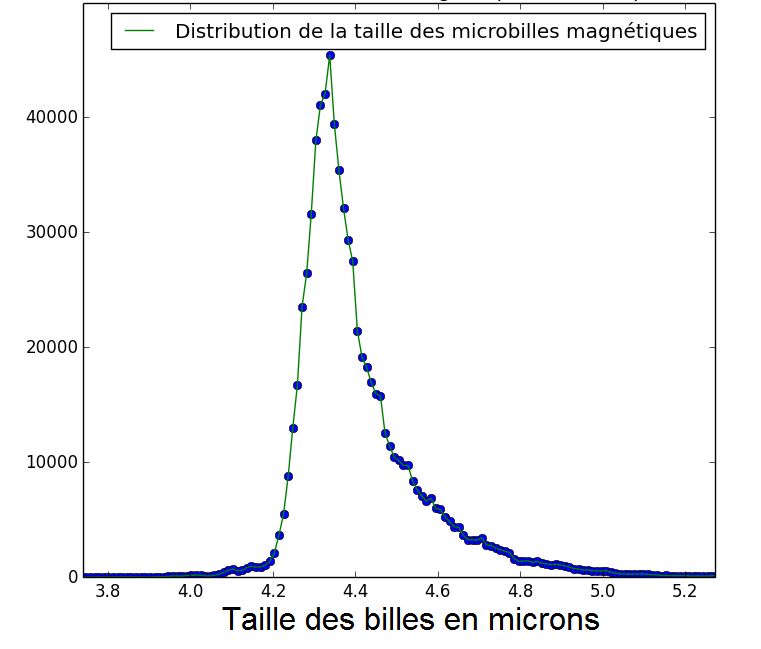
\includegraphics[scale=0.5]{Taille_des_billes.png}
		\caption{Fonction de distribution de taille des billes magnétiques utilisées dans 191 expériences de pinces. Pour chaque expérience, lorsque la bille est suivie par le logiciel d'analyse d'image, son grand axe et son petit axe sont mesurés pour chaque temps. La fonction est asymétrique car lorsque la bille n'est pas tout à fait au point, son diamètre apparaît plus grand.}
\end{figure}		 
		
		\subsubsection{\'Electroaimant}
		\subsubsection{Montage sous microscope}
	\subsection{Calibration}
	\subsection{Protocole de renforcement}
	\subsection{Dépouillement des vidéos}
		\subsubsection{ImageJ}
		\subsubsection{Icy}
\section{\'Etirement}
	L'objectif de ce dispositif est de soumettre les cellules à une déformation constante pendant plusieurs heures et de les observer en fluorescence pendant l'étirement sur un microscope inversé. 
	\subsection{Description de l'étireur}
	Pendant ma thèse j'ai conçu les plans de cet étireur de cellules qui a ensuite été réalisé par l'atelier du laboratoire. Il est composé de trois parties principales : la cuve, le support de lamelle et le plot. Toutes les parties de l'étireur sont en plastique, le plot étant transparent pour laisser passer la lumière du condenseur. L'étireur à une symétrie cylindrique autour d'un axe vertical. 
	\subsubsection{La cuve}
	La cuve doit remplir deux fonctions : contenir le milieu de culture nécessaire aux cellules et permettre l'observation de celles-ci au microscope inversé. Elle est composée de deux pièces trouées en leur centre qui se vissent l'une dans l'autre. Au niveau de l'ouverture destinée à l'observation, on place une lamelle de verre de 30 mm de diamètre dont le contour a été préalablement enrobé dans du téflon souple. Cette lamelle de verre est enserrée entre les deux pièces de façon à former une cuve étanche dont le fond transparent permet l'observation.
	\subsubsection{La lamelle de PDMS} 
	Les cellules adhèrent à une lamelle de PDMS réticulé élastique recouverte de fibronectine. Cette lamelle est maintenue par le support et déformée par le plot qui la pousse vers le bas. 
	Le PDMS est fabriqué à partir d'un mélange 90\% PDMS et 10\% de réticulant. On place alors 1,8g du mélange dans une boite de Petri de XX mm de diamètre et on l'étale jusqu'à la recouvrir entièrement de manière homogène. La masse est choisie de façon à ce que le PDMS étalé fasse 0,3mm d'épaisseur. Les boîtes recouvertes de PDMS sont alors placées toute la nuit dans un incubateur à 60\degres  C pour réticuler le gel. À l'aide d'un emporte-pièce, des disques de 30mm sont alors découpés dans les boîtes.

		
	\subsubsection{Le support}
	Le support est la pièce de serrage de la lamelle de PDMS sur laquelle sont cultivées les cellules. La lamelle de PDMS est placée entre deux anneaux plats de téflon d'un millimètre d'épaisseur qui sont destinés à homogénéiser la pression exercée sur la lamelle par la pièce de serrage. L'ensemble est posé sur un support de hauteur variable (1 mm ou 3mm) qui va déterminer l'étirement maximal possible, et serré par une pièce qui se visse dans le support. 
	Cette pièce doit maintenir fermement les bords de la lamelle en place tandis que le centre est étiré par le plot. 
	\subsubsection{Le plot}
	Le plot transparent est maintenu dans une pièce qui se visse à l'intérieur de la cuve. Le vissage va faire descendre le plot, qui va ainsi étirer la lamelle en la rapprochant du fond de la cuve et donc de l'objectif du microscope. 
	L'utilisation du support de 1mm ou de 3mm permet de fixer la lamelle de PDMS à différentes hauteurs, et donc pour un même abaissement du plot d'étirer plus ou moins la lamelle. Il existe deux diamètre de plots cylindriques : 10mm et 15mm, qui permettent également de régler l'étirement subit par le PDMS. 
	\subsection{Calibration de l'étireur}
	
	Un modèle géométrique simple permet d'estimer rapidement l'augmentation de la surface de la lamelle de PDMS en fonction du diamètre et de l'enfoncement du plot. 
	
	
	
	
	Afin de le comparer à l'étirement réel subi par la lamelle de PDMS, des lamelles ont été recouvertes de Pluronics, puis exposées à un rayonnement UVC à travers un masque de quartz contenant un grand nombre de carrés de taille connue formant un quadrillage. Puis les lamelles ont été recouvertes de fibronectine fluorescente, qui ne pouvait adhérer qu'aux endroits non éclairés par les UV. 
	
	\paragraph{Ingrédients : }
	\begin{itemize}
	\item une lamelle de PDMS vierge
	\item Pluronics
	\item Fibronectine Cy3
	\item un masque en quartz 
	\item une lampe UVC
	\end{itemize}
	
	\paragraph{Protocole}
	\begin{enumerate}
	\item Préparez une solution de Pluronics 0,2\% en masse
	\item Laissez incuber 1 ml de la solution de Pluronics pendant une heure à température ambiante
	\item Rincez au PBS, puis à l'eau, laissez sécher
	\item Exposez la lamelle derrière le masque aux UVC pendant 7 minutes
	\item Diluez 4 \micro g de fibronectine fluorescente dans 1 ml de PBS
	\item Laissez la solution de fibronectine incuber 30 minutes à 37 \degres C sur la lamelle, à l'abri de la lumière
	\item Rincez au PBS et stockez à 4 \degres C dans le PBS, à l'abri de la lumière
\end{enumerate}		
	
	Nous avons ainsi obtenu des lamelles recouvertes d'un quadrillage visible en microscopie de fluorescence. Ce quadrillage a été observé avant et après étirement, et l'étirement a alors été mesuré à partir de la formation du quadrillage
	
	Les images nous montrent que la déformation du PDMS par le plot est radiale et uniforme, et que le modèle géométrique le plus simple décrit bien quantitativement la déformation subie. 
	
	\subsection{Le microscope confocal}
	
	Pour les expériences d'étirement, il était nécessaire d'utiliser le microscope confocal du laboratoire car il était le seul à disposer d'une platine motorisée, de 4 lasers et des filtres automatisés. Cependant, l'étireur impose d'avoir un plan focal situé à une grande distance de l'objectif, ce qui impose l'utilisation d'un objectif à air à grande distance de travail. Cela nous interdit malheureusement de profiter de la fonctionnalité du confocal qui est de faire des images en 3D. 
	
	Les observations en fluorescence contiennent donc nécessairement une intégration du signal selon l'axe vertical, ce qui implique que les endroits où la cellule est épaisse apparaissent comme plus lumineux que les endroits où elle est fine. 
	
	Il en ressort que la zone du noyau, la plus épaisse de la cellule, est presque toujours plus lumineuse que les bords de la cellules qui sont très fins. 
	Il peut alors se révéler peu pertinent de comparer la fluorescence du cytoplasme en entier et la fluorescence du noyau lorsqu'on veut comparer la concentration d'une protéine fluorescente de part et d'autre de la membrane nucléaire.
	
	C'est pourquoi il peut être intéressant de regarder non seulement toute la cellule, mais également une zone péri-nucléaire, d'épaisseur semblable au noyau. Entre le noyau et la zone péri-nucléaire, on compare des luminosités à épaisseur fixée.
	
	\paragraph{Description générale}
	
	Le microscope confocal est composé : 
	\begin{itemize}
	\item d'un microscope inversé Olympus IX81
	\item de 4 lasers de puissance réglable Andor Laser Combiner 400 series
	\item d'une roue motorisée de 10 filtres Sutter Lambda 10B Controller
	\item d'un disque rotatif Yokogawa CSUX1
	\item d'une platine motorisée Prior Proscan II
	\item d'un système piézo de réglage pour l'axe Z Andor APZ-100
	\item d'une caméra Andor IXON+
	\item d'un ordinateur avec le logiciel constructeur IQ2 pour contrôler l'ensemble
	\item d'une enceinte thermalisée par un Cube 2 de Life Imaging Services
\end{itemize}	 

Dans les expériences décrites, sauf indications contraires, il sera utilisé avec un objectif 20X Olympus à grande distance de travail. 

Quatre configurations d'observation ont été utilisées pour la fluorescence : 
\begin{itemize}
\item[Rouge profond] : Laser d'excitation 640nm et filtre 685nm
\item[Rouge] : Laser d'excitation 561nm et filtre 607nm
\item[Vert] : Laser d'excitation 488nm et filtre 525nm
\item[Bleu] : Laser d'excitation 405nm et filtre 465nm
\end{itemize}
	
	\subsection{Protocole d'étirement observé en direct}
	Les cellules sont ensemencées sur des lamelles de PDMS préalablement recouvertes de fibronectine. Afin d'améliorer l'efficacité de transfection, dans le protocole final, les cellules sont transfectées avec la nanofectine pendant 6h avant d'être rincées décollées, comptées et ensemencées à raison de 110 000 cellules par lamelle. 
	
	Après avoir mené un certain nombre d'expériences, nous avons constaté que la sensibilité de MRTF-A à la stimulation par le sérum est telle que le fait de remplacer le milieu de culture dans lequel les cellules baignaient depuis 24h par du milieu de culture neuf provoque des modifications non négligeables de la localisation de MRTF-A dans les cellules. Il est donc essentiel de conserver le même milieu de culture tout au long de l'expérience. 
	
	Après ensemencement et adhésion, les lamelles de PDMS peuvent être montées à l'avance sur le support et maintenues dans 5 à 7ml de milieu de culture blanc (5ml pour l'étirement 10\% et 7ml pour 30\%). 
	
	Juste avant l'expérience, la lamelle et le milieu de culture sont montés dans le reste de l'étireur et 1,5\% d'HEPES sont alors ajoutés pour tamponner l'acidité du milieu pendant la durée de l'expérience. L'étireur complet est alors placé sur la plate-forme du microscope et observé à l'aide d'un objectif 20X (trouver les caracs de l'objectif). Les cellules sont observées en lumière blanche et en fluorescence une première fois avant étirement brièvement, afin d'avoir une idée de l'état de départ des cellules. 
	
	En vissant le plot, on étire alors la lamelle rapidement en quelques secondes jusqu'à la déformation souhaitée. On cherche alors des cellules exprimant la MRTF-A GFP. À chaque fois qu'une ou plusieurs cellules sont visibles dans un champ, on enregistre la position de la platine motorisée. Toutes les 5 à 10 minutes, on retourne observer toutes les cellules répertoriées afin de suivre l'évolution de la localisation de MRTF-A au cours du temps. De nouvelles cellules sont recherchées jusqu'à 40 minutes après l'étirement et l'observation est ensuite maintenue pendant 2h après l'étirement. 
	
	
	\subsection{Protocole d'étirement fixé}
	
	Le protocole d'étirement avec observation en direct ne nous permet pas d'observer la population de cellules à des instants courts, car il faut du temps pour retrouver un nombre suffisant de cellules. De plus, l'observation de l'état du cytosquelette en direct est difficile car les différents marqueurs disponibles perturbent trop le système : la surexpression d'actine lors de la transfection avec une actine Mcherry modifie de manière très visible l'équilibre entre MRTF-A et l'actine G, la LifeAct RFP est exprimée tellement intensément que sa fluorescence empiète sur celle de MRTF-A GFP. 
	
	Fixer les cellules nous permet d'avoir un marquage quadrichrome : la F-actine en rouge-profond grâce à la phalloïdine, la G-actine en rouge grâce à la DNaseI, MRTF-A GFP ou anticorps anti-MRTF-A en vert et l'ADN du noyau en bleu grâce au DAPI. 
	
	Pour une expérience d'étirement fixé, on prépare une boîte de C2C12 proches de la confluence (60-70\%) transfectées si l'on veut observer la MRTF-A GFP. Elles sont ensemencées ensemble sur 6 lamelles de PDMS dans une plaque 6 puits dans 3ml de milieu de culture 24h avant le début de l'expérience. Le lendemain, une de ces lamelles est montée sur le support, rincée au PBS et fixée immédiatement, c'est la lamelle témoin. Les autres lamelles sont successivement étirées, laissées à l'incubateur pendant un temps donné, puis démontées, rincées et fixées immédiatement. On obtient ainsi pour un même étirement une lamelle à t=0 et 5 lamelles à différents temps après étirement (par exemple 5,10,20,30,60 minutes après étirement). 
	
	Ces lamelles sont ensuite marquées dans les 4 couleurs suivant un protocole strictement identique, et observées avec des paramètres strictement identiques (intensité du laser, temps d'exposition \dots) au microscope, afin de pouvoir comparer quantitativement les intensité de fluorescence d'une lamelle par rapport aux autres. 
	

	\subsection{Dépouillement des images}
	\subsubsection{\'Etirement observé en direct, traitement qualitatif}
	On obtient après une observation en direct d'étirement typique une vingtaine de série d'images de cellules observées pendant 120 minutes après étirement. 
	Les images sont observées grâce à ImageJ, qui nous permet de reconstituer une pile d'images en 4 dimensions (x,y,temps et couleur). On peut alors observer qualitativement à l'\oe il s'il y a plus de MRTF-A GFP dans le noyau, dans le cytoplasme, ou si c'est homogène. 
	
	Toutes les données finales sont destinées à être stockées dans une base de donnée SQL. Cette forme de stockage de données permet de sélectionner et de trier les données en fonction de nombreux critères à la fois quantitatifs et qualitatifs. Pour remplir la base de donnée, j'ai également créé une interface en Python. Cette interface récupère dans les métadonnées des images prises au microscope les temps auxquelles ces images ont été prises. L'utilisateur peut alors remplir pour chaque temps la localisation principale de MRTF-A dans la cellule : Nucléaire, Homogène ou Cytoplasmique. 
	Pour chaque champ d'observation, il note également le nombre de cellules visibles dans le champ, ce qui permet d'évaluer la densité locale de cellules. 
	
	Dans cette base de données, on retrouve alors pour chaque cellule la localisation de MRTF-A au cours du temps écoulé depuis l'étirement, l'étirement, le passage, le nombre de cellules présentes dans chaque champ, et l'expression en Actine Mcherry.
	\subsubsection{\'Etirement fixé, traitement quantitatif}	
	
	Pour chaque lamelle fixée, on obtient une série d'images en 5 couleurs : rouge profond, rouge, vert, bleu et lumière blanche. 

À partir des images en rouge profond et en rouge, on peut créer une nouvelle image en divisant chaque valeur de pixel rouge profond par la valeur en pixel rouge. On obtient alors une image représentant dans l'espace le rapport entre le signal de la F-actine et celui de la G-actine.

Pour chaque cellule, on procède alors ainsi : 
\begin{itemize}
\item Si la cellule est isolée, on utilise un seuillage sur l'image en rouge profond pour sélectionner le contour de la cellule
\item Si la cellule est collée à une autre cellule, il faut sélectionner le contour à la main
\item On mesure alors la valeur moyenne des pixels dans cette zone, son aire, ses paramètres géométriques\dots
successivement en rouge profond (F-actine), en rouge (G-actine) et en rapport (F/G). 
\item On fait un seuillage sur l'image en DAPI afin de sélectionner le contour du noyau
\item On mesure alors les valeurs dans le noyau en rouge profond, rouge, vert et en rapport F/G. 
\item On sélectionne enfin une zone péri-nucléaire d'intensité homogène, qui correspond à une zone d'épaisseur proche de celle du noyau
\item On mesure alors les valeurs en rouge et en vert dans cette zone
\end{itemize}	
	
	On obtient alors des tableaux de données contenant les valeurs moyennes d'intensité pour la phalloïdine, la DNase et la MRTF-A (GFP ou endogène) et les aires des cellules et de leurs noyaux. 
	
	
\end{document}